\documentclass[preprint]{aastex}  % USE THIS TO MAKE BIB, THEN FORMAT USING EMULATEAPJ
%\documentclass[twocolumn,numberedappendix]{emulateapj}
\shorttitle{Transit Dish for 21cm Intensity Mapping}
\shortauthors{XXX Authors}

\usepackage{amsmath}
\usepackage{graphicx}
\usepackage[figuresright]{rotating}
%\usepackage{rotating}
\usepackage{natbib}
%\usepackage{pdflscape}
%\usepackage{lscape}
\citestyle{aa}

\newcommand{\BigO}[1]{\mathcal{O}(#1)}
\def\k{\mathbf{k}}
\def\r{\mathbf{r}}
\def\V{\mathbb{V}}
\def\At{\tilde{A}}
\def\Vt{\tilde{V}}
\def\Tt{\tilde{T}}
\def\tb{\langle T_b\rangle}

\begin{document}
\title{A Transit Dish Design for High-Redshift 21cm Intensity Mapping Experiments}

\author{
%Aaron R. Parsons\altaffilmark{1,2},
%Adrian Liu\altaffilmark{1},
%James E. Aguirre\altaffilmark{3},
%Zaki S. Ali\altaffilmark{1},
%Richard F. Bradley\altaffilmark{4,5,6},
%Chris L.  Carilli\altaffilmark{7},
%David R. DeBoer\altaffilmark{2},
%Daniel C. Jacobs\altaffilmark{8},
%David F. Moore\altaffilmark{3},
%Jonathan C. Pober\altaffilmark{1},
}

%\altaffiltext{1}{Astronomy Dept., U. California, Berkeley, CA}
%\altaffiltext{2}{Radio Astronomy Lab., U. California, Berkeley, CA}
%\altaffiltext{3}{Dept. of Physics and Astronomy, U. Pennsylvania, Philadelphia, PA}
%\altaffiltext{4}{Dept. of Electrical and Computer Engineering, U. Virginia, Charlottesville, VA}
%\altaffiltext{5}{National Radio Astronomy Obs., Charlottesville, VA}
%\altaffiltext{6}{Dept. of Astronomy, U. Virginia, Charlottesville, VA}
%\altaffiltext{7}{National Radio Astronomy Obs., Socorro, NM}
%\altaffiltext{8}{School of Earth and Space Exploration, Arizona State U., Tempe, AZ}
%\altaffiltext{9}{Square Kilometer Array, South Africa Project, Cape Town, South Africa}
%\altaffiltext{10}{Cavendish Lab., Cambridge, UK}

\begin{abstract}
\end{abstract}

\section{Introduction}

\begin{itemize}
\item importance of frequency smoothness
\item collecting area
\end{itemize}

\section{Background}
\label{sec:background}

\begin{itemize}
\item $\tau$-modes, wedge, EoR window
\item geometric interpretation of $\tau$-modes
\end{itemize}

\section{Geometric Constraints}
\label{sec:geometry}

\begin{itemize}
\item first principles of EoR window, how that maps to a specification for design
\item cost analysis
\item critically constrained design
\item symmetric on-axis parabaloid, for reasons of symmetry in polarization response
\end{itemize}

\section{Design and Construction}
\label{sec:design}

\subsection{bent pipes as approximation to parabola}

\begin{figure}[H]
	\begin{center}
	
\includegraphics[width =\textwidth]{empty}
	\caption{THIS FIGURE SHOWS THE ANALYSIS ON PARABOLA
\label{Fig:} }
	\end{center}
\end{figure}


\subsection{faceting}
\begin{figure}[H]
	\begin{center}
	
\includegraphics[width =\textwidth]{empty}
	\caption{THIS FIGURE SHOWS THE PHOTGRAMMRY ANALYSIS 
\label{Fig:} }
	\end{center}
\end{figure}

\subsection{sheiding}
The panels across the dish surface are made out of 6 different dimensions of galvanized wire cloth $\frac{1}{4}$"; employing different dimensions at different heights to reduce the surface bumps produced during installation.

\subsection{splash cone}
\begin{figure}[H]
	\begin{center}
	
\includegraphics[width =\textwidth]{empty}
	\caption{THIS FIGURE SHOWS THE SPLASH CONE STRUCTURE
\label{Fig:} }
	\end{center}
\end{figure}

\subsection{hub}
The central hub has an overall diameter of 37", the inner sono tube has an interior diamater of 18", the outer sono tube has an interior diameter of 36". The launch angle of the spar sleeves is $+2.86^{\circ}$ from the inner sono tube to the outer sono tube, the supporting sleeves (botton sleeves) do not have any launch angles.


\subsection {feed suspension}
The feed suspesnsion mechanism consists of a back plane made out of wire cloth and $\frac{3}{4}$" schedule 40 white PVCs bolted on a metal structure, and a mast from the metal structure connects the dipole feed to the back screen. The whole feed structure is suspended above the hub by attaching kevlar wires from the three telephone poles to the back of the metal structure. 

Each telephone pole has a reel with kelvar ropes wrapped, adjustments to feed height can be made by cranking the reels.


\subsection{material, PVC selection}
The dish structure is made out of schedule 40, white PVCs to minimize the bending effect under sunlight exposure; PVCs are subject to thermal contraction and expansion with a linear thermal coefficient of $50.4\times10^{-6}\ \frac{m}{m^{\circ}C}$.


\begin{itemize}
\item bent pipes as approximation to parabola 
\item faceting
\item shielding
\item splash cone
\item hub 
\item feed suspension (feed with mast, back screen by kevlar wire)
\item materials, PVC selection 
\item design lifetime (wood, PVC)
\end{itemize}

\section{Simulated Performance}
\label{sec:sim}

\subsection{Beam Pattern}

\begin{figure}[H]
	\begin{center}
	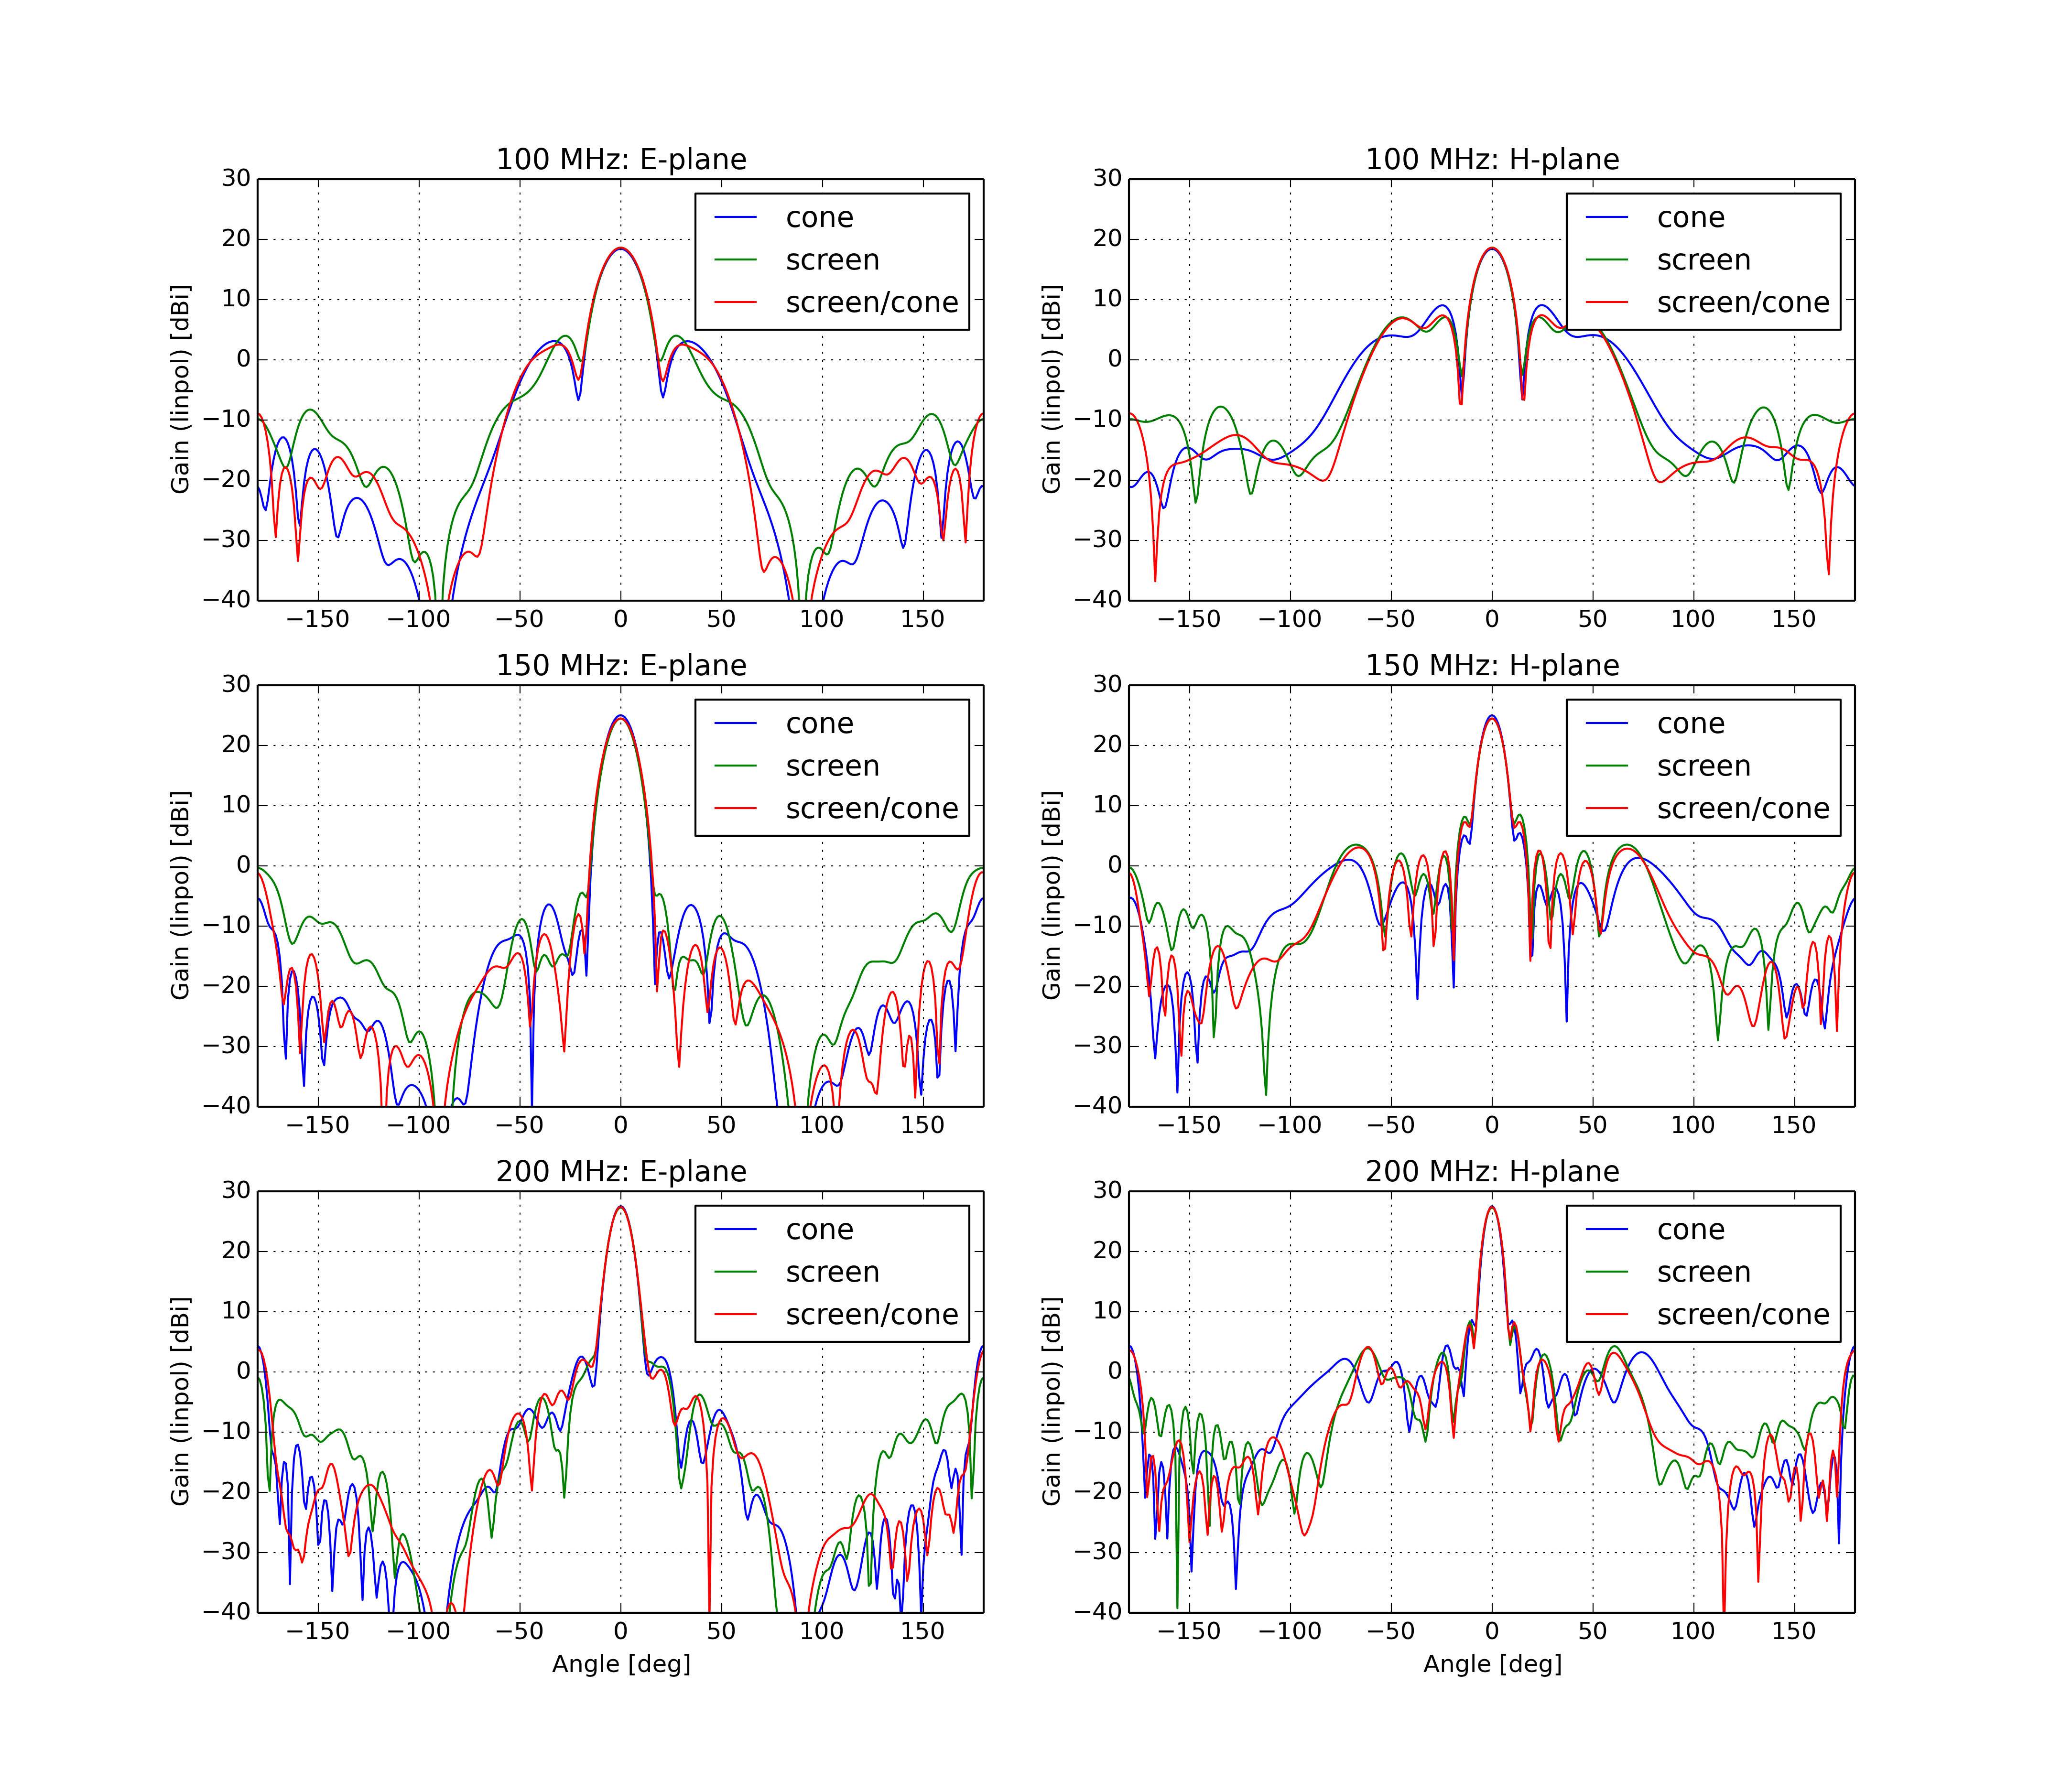
\includegraphics[width =\textwidth]{./dish_plots/Beampatterns_cone}
	\caption{THIS FIGURE SHOWS THE BEAM PATTERN 
\label{Fig:} }
	\end{center}
\end{figure}

\begin{itemize}
\item beam pattern
\item delay performance (E-M modeling)
\end{itemize}

\section{Fabrication and Deployment}
\label{sec:deploy}

\begin{itemize}
\item lessons/principles
\item process to precision to specifications on precision
\end{itemize}


\section{Reflectometry Test Setup}
\label{sec:reflect}
During the contruction process for the HERA prototype, we use Time Domain reflectometry(TDR) to measure the reflections on the dish as a function of time due to impedance mistmatch between the feed electronics and the sky signal. The feed characteristic impedance from the VNA and cable is 50 $\Omega\times4 $(4:1 passive balun at each dipole) and that of the free space $120\pi\Omega$. Each polarization is fed into one port connected to the VNA which provides a frequency swept signal and inverse Fourier transform is then performed.  In this prototype, the focal length is $4.5$m, thus for 2 reflections, i.e. 4 crossings attenuation is 59.0ns in time domain.


\subsection{Choice of Hardware}
The dipole feed element consists of the PAPER feed, a mating board, one 4:1 passive balun for each polarization, 50$\Omega$ LMR400 cables of length 10m where the singal attenuation over 10m is ~ 0.5dB at 150MHz. 
The cables are connected to the two ports of an Agilent VNA ES8753 for reflectometry measurements. 


\subsection{Calibration of VNA}
Calibration is performed prior to taking measurements to eliminate the effects caused by cables and connectors. Performing calibration shifts the reference plane to the SMA connectors of the cables that are connecting the baluns with zero phase, zero loss and zero mistmatch, the measurements taken are showing only the effects of the feed and baluns under different configurations. The full two port calibration is done by attaching the calibration standards (Short, Open, Load, and Through) to the end of the $50\Omega$ cables, the VNA calculates the correction coefficients by calibrating out at the calibration standards' impedances and applies the coefficients subsequently to each measurements.

\subsection{Feed Height Test}
The feed height test is carried out at three different heights above the dish: $67"$, $10'3.5"$, and $14'0.5"$.
See Delay Spectrum for Configurations under result section for images


\subsection{Configurations}
The measurements are taken with 401 data samples between 50MHz to 1000MHz, giving a time resolution of 1.05ns; each set of data is averaged by 16 measurements for higher SNR. 









(SELF NOTE)April 16
@ 14'3" 
$no_cone1 $= containing data taken without cone with 1 metal sheet
@14'6"
set3- set4: measuremnets with cone, 1 metal sheet covering the entrance to the dish, covering panel A



May 5th stuff
@ height 14' 6"
Dish without cone, with screen
set1- set2: measurements without cone, 2 metal sheets covering the entrace to the dish, covering panel A, B
set5- set6: measurements with cone, 2 metal sheets covering the entrance to the dish, covering panel A, B

\subsection{Window Functions}
To deal with real-life situations of a finite bandwidth which results in spectral leakage in time domain,  the Kasier-Bessel window is applied to the frequency domain data prior to the inverse Fourier transform in order to increase the dynamic range of the measurements in time domain; the disadvantage however, is the widening of space between data points.


\begin{figure}[H]
	\begin{center}
	
\includegraphics[width =\textwidth]{empty}
	\caption{PUT FIGURE SHOW WINDOW 
\label{Fig:} }
	\end{center}
\end{figure}


\begin{itemize}
\item reflectometry 
\item hardware 
\item calibration of the good
\item feed height test
\item configurations
\item window function used in delay transform
\end{itemize}

\section{Results}
\label{sec:results}
\subsection{Delay Spectrum for Configurations}
Using TDR 

\begin{figure}[H]
	\begin{center}
	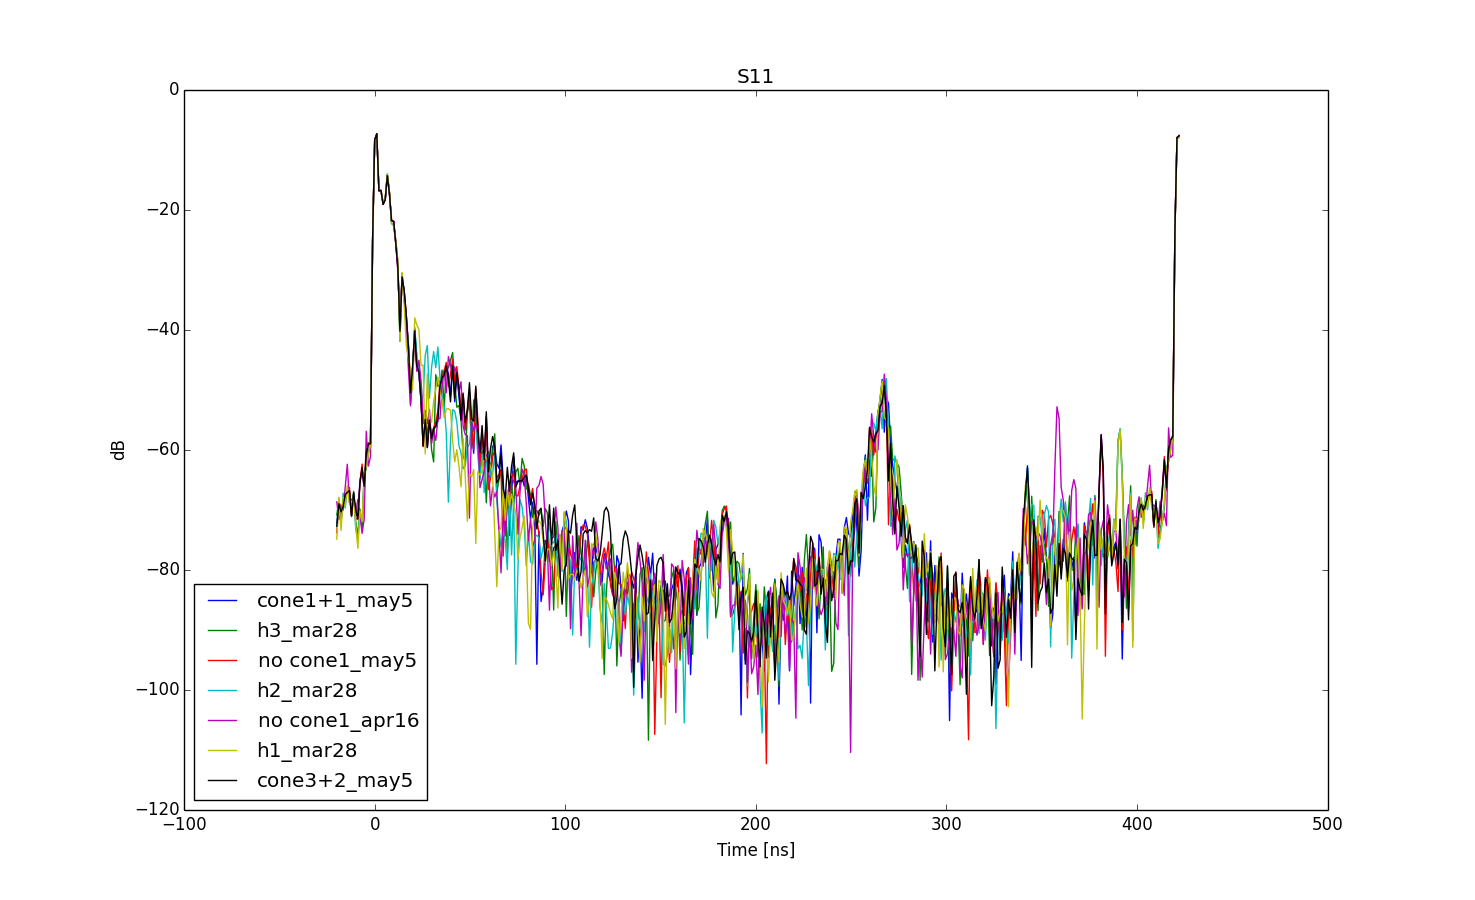
\includegraphics[width =\textwidth]{./reflectometry_plots/configcompare}
	\caption{Shows mar28 height tests, apr16, may5 cone test
\label{Fig:} }
	\end{center}
\end{figure}
\begin{figure}[H]
	\begin{center}
	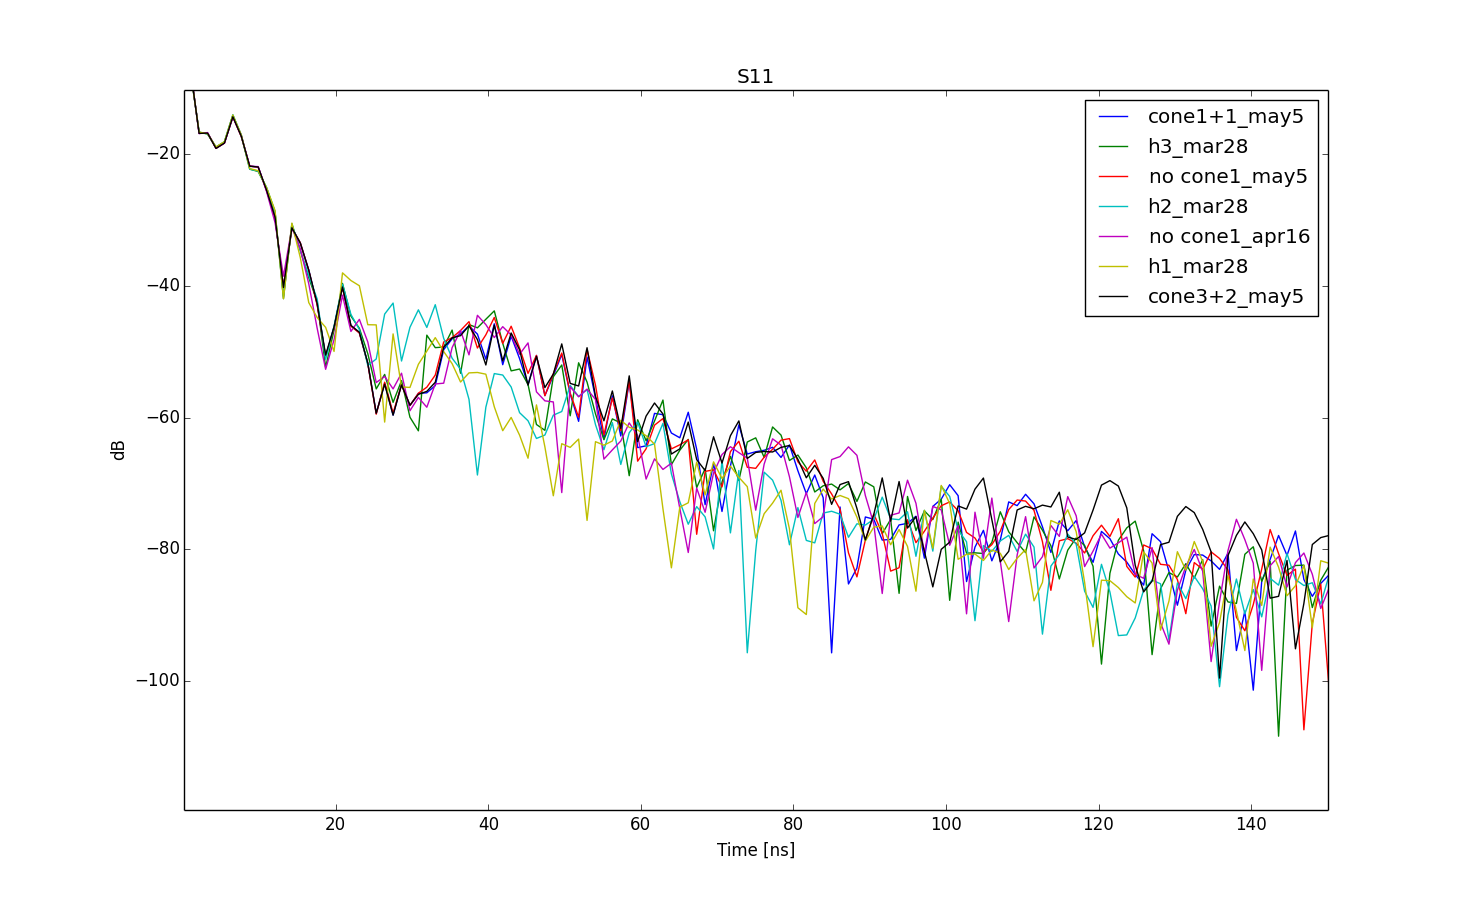
\includegraphics[width =\textwidth]{./reflectometry_plots/configcompare10-150ns}
	\caption{Shows mar28 height tests, apr16, may5 cone test zoomed on 10-150ns, can see height test changed the delay
\label{Fig:} }
	\end{center}
\end{figure}

\begin{figure}[H]
	\begin{center}
	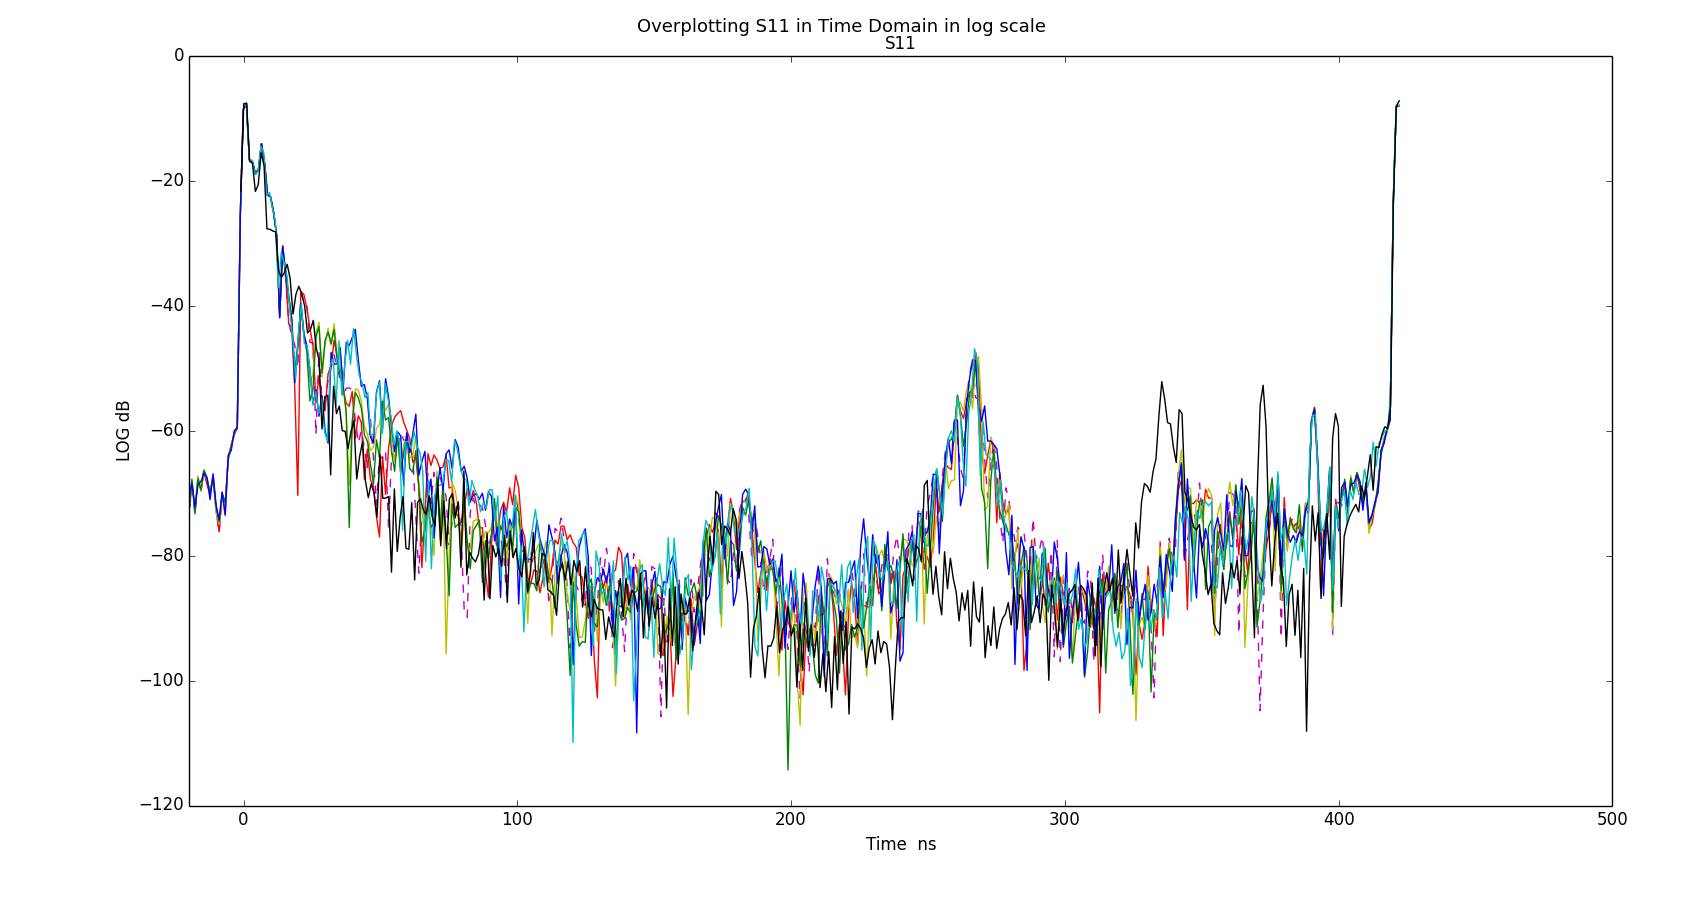
\includegraphics[width =\textwidth]{./reflectometry_plots/Mar28/s11all-mar28mix17set1}
	\caption{Shows mar28 height tests, apr16, may5 cone test and test not on dish, shows bump is reflection due to surroundings.
\label{Fig:} }
	\end{center}
\end{figure}

May 5th stuff
@ height 14' 6"
mountain bumps ~ 60' - 80'
Dish without cone, with screen
set1- set2: measurements without cone, 2 metal sheets covering the entrace to the dish, covering panel A, B
set5- set6: measurements with cone, 2 metal sheets covering the entrance to the dish, covering panel A, B

\begin{figure}[H]
	\begin{center}
	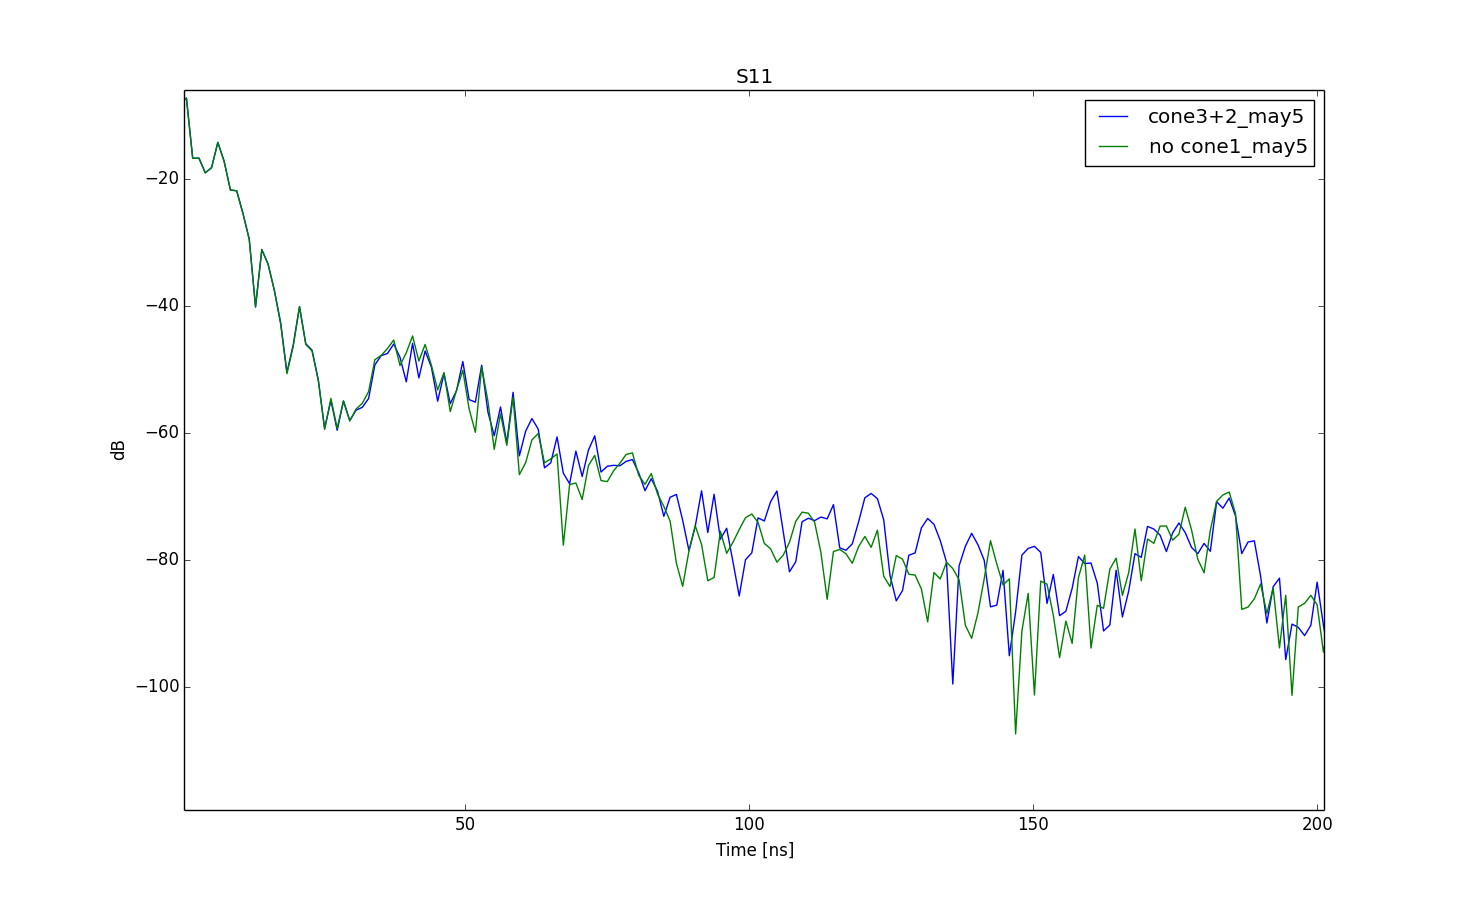
\includegraphics[width =\textwidth]{./reflectometry_plots/May5/set1vsset3zoom}
	\caption{CONFIG 1
\label{Fig:} }
	\end{center}
\end{figure}
=====

April 16
@ 14'3" 
$no_cone1$ = containing data taken without cone with 1 metal sheet
@14'6"
set3- set4: measuremnets with cone, 1 metal sheet covering the entrance to the dish, covering panel A
\begin{figure}[H]
	\begin{center}
	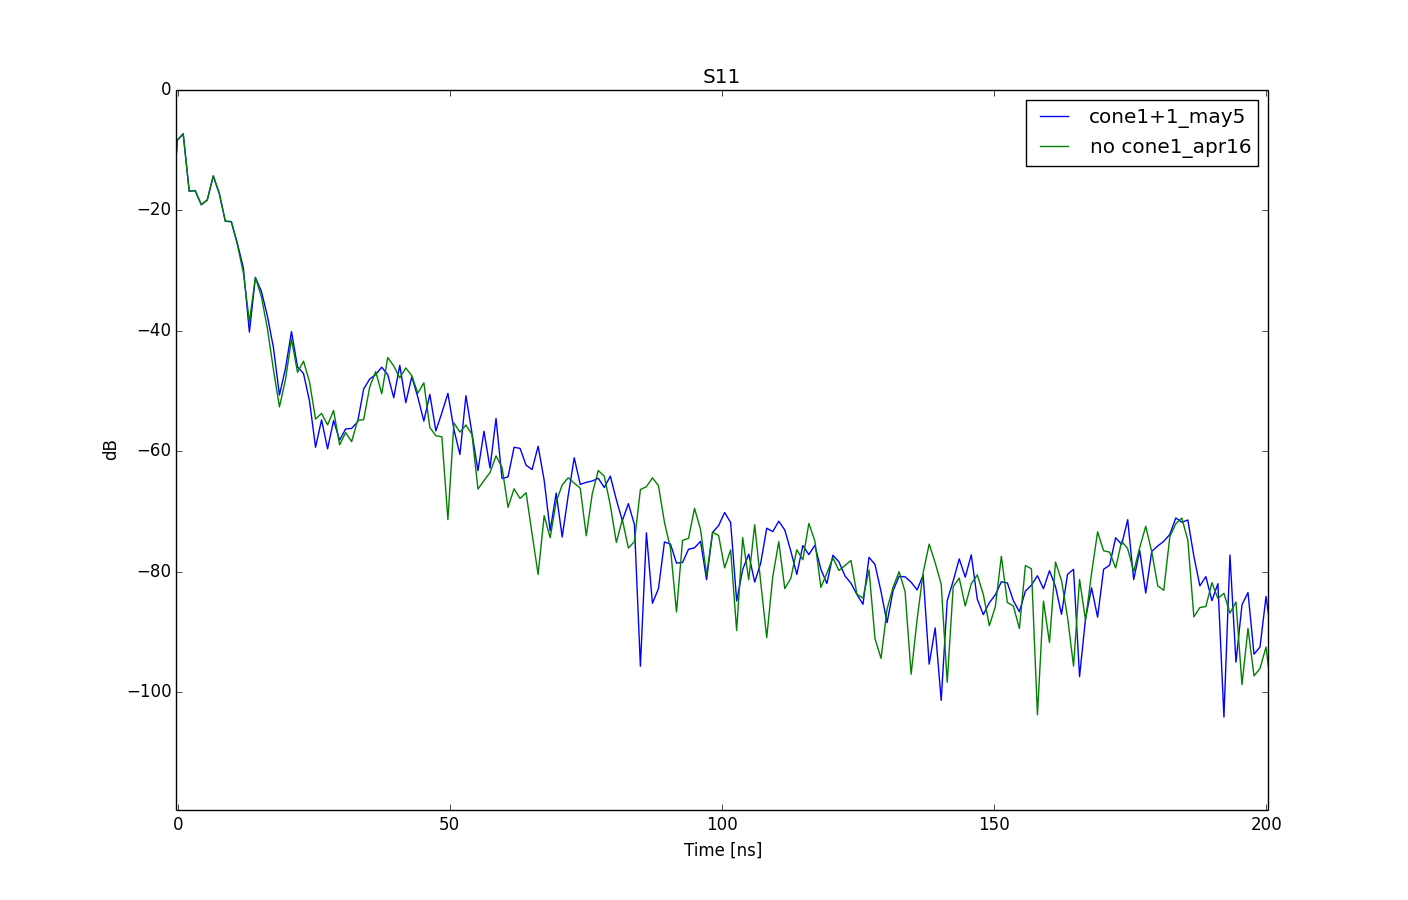
\includegraphics[width =\textwidth]{reflectometry_plots/May5/nocone_vs_set3zoom}
	\caption{CONFIG 2
\label{Fig:} }
	\end{center}
\end{figure}

\begin{figure}[H]
	\begin{center}
	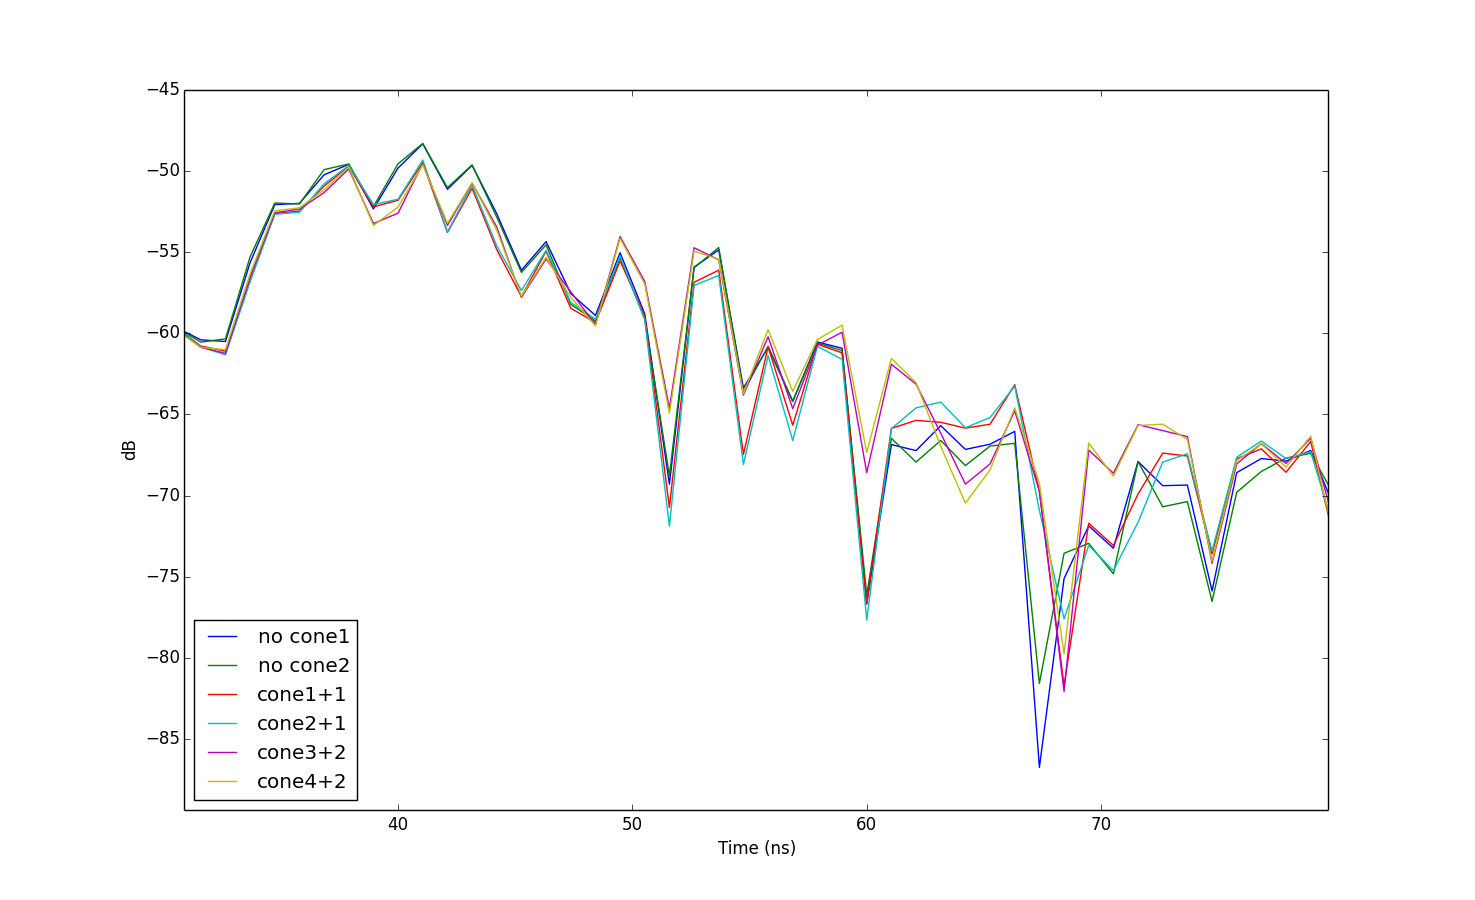
\includegraphics[width =\textwidth]{reflectometry_plots/May5/S11_1st2nd_refl}
	\caption{Shows cone VS no cone, combine 2 plots above, apparent difference cone make, but needs redesign for better backlobe minimization as seen from ~48ns.
\label{Fig:} }
	\end{center}
\end{figure}

========
dish different heights
Mar 28
h1 = 67"
h2 = 10'3.5"
h3 = 14'0.5"

\begin{figure}[H]
	\begin{center}
	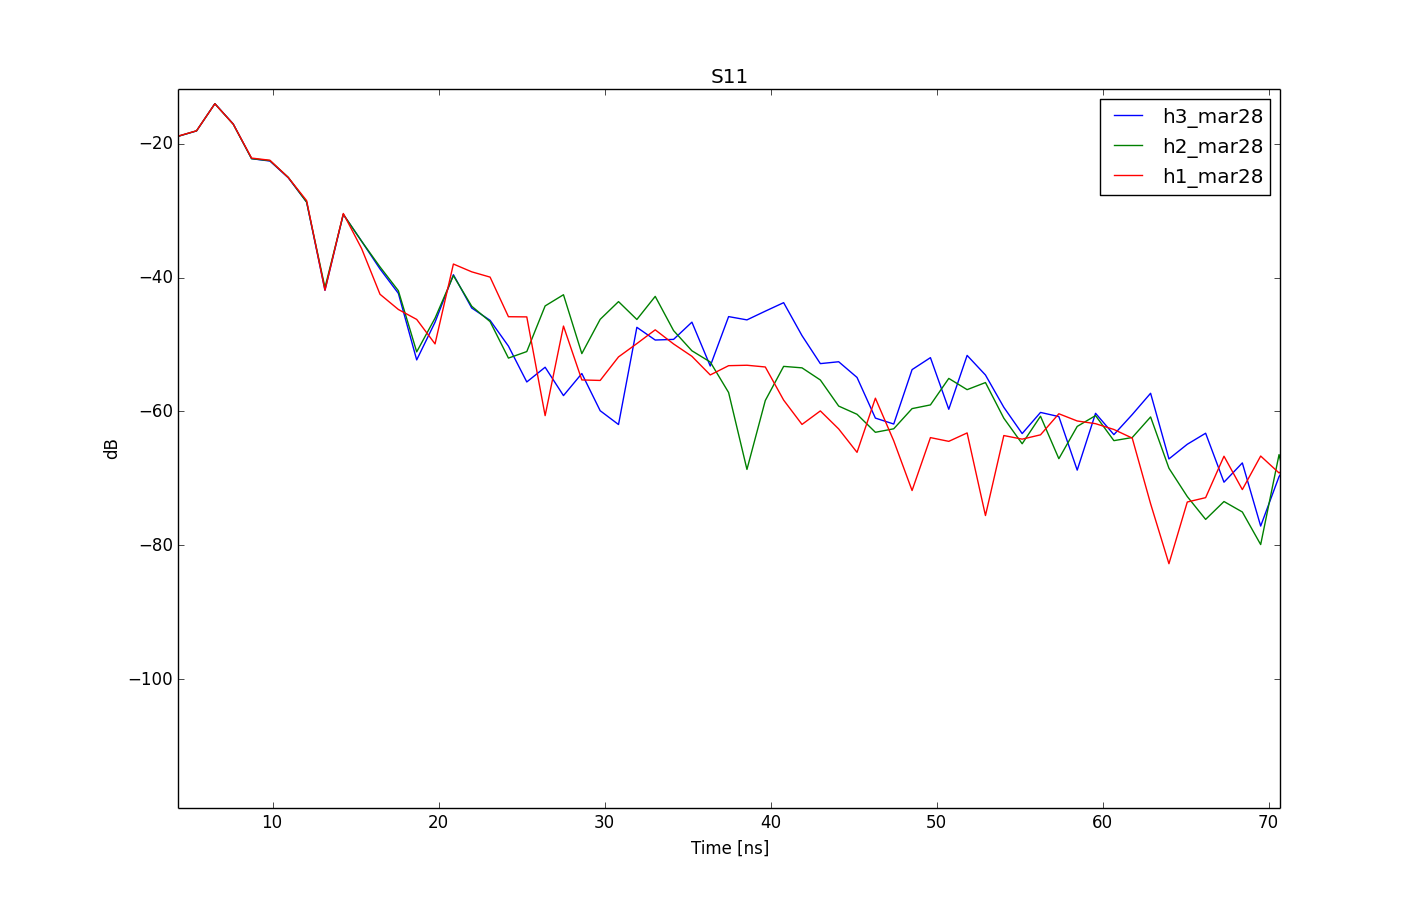
\includegraphics[width =\textwidth]{reflectometry_plots/Mar28/height_test_zoom}
	\caption{height test zoomed
\label{Fig:} }
	\end{center}
\end{figure}



\subsection{Cone test}
$\>$ show May 5th cone helped on reduce backlobe, see section \ref{label:reflect}

\subsection{RFI investigation}
Replacing the passive balun by the PAPER active balun and mating board, $75 \Omega$ cables are fed into the receiver, and the receiver outputs $50\Omega$ through the LMR 400 cables to the Agilent E4407B spectrum analyzer. 401 points, 100MHz - 200MHz, average by xx measurements, sweep time is xx ms, bandwidth resolution is xx kHz.

What are the gains for the balun, the receiver?

\begin{figure}[H]
	\begin{center}
	
\includegraphics[width =\textwidth]{empty}
	\caption{SHOW SPECTRUm ANALYZER 100MHz - 200 MHz plot, radio stations, VHF showed up
\label{Fig:} }
	\end{center}
\end{figure}


\subsection{How well did we place everything}
Resurvery the center for hub after telephone poles were stabilized in the ground. The telephone poles have varying diamater and along the length. 

The surrounding posts are not equidistant to the center of the hub; within ~5' between maximum post to center distance and minimum post to center distance.

 

\begin{itemize}
\item delay spectrum for configurations
\item cost
\item photos of constructed element
\item XXX hook up receiver and to a sky test?
\item measured parabolicity
\item why were we right in the antenuation per reflection?
\item does the cone help?
\item how well did we place everything?
\item ways to ensure spec in field
\item mention extender as unnecessary in flat deployments
\end{itemize}

\section{Conclusion}
\label{sec:conclusion}

\begin{itemize}
\item relevance to HERA, project cost
\item link Pober et al. (2014) sensitivity/science
\item polarization matching
\item frequency coverage, need for a feed re-design.
\end{itemize}

\section{Acknowledgment}

We would like to thank SKA-SA for the site infrastructure, maintenance, and observing support
that has made this work possible, as well as the significant efforts of the staff at
NRAO's Green Bank and Charlottesville sites.  AP would like to thank M. McQuinn and A. Lidz
for helpful discussions and ionization models.
The PAPER project is supported
by the National Science Foundation (awards 0804508,
1129258, and 1125558), and a generous grant
from the Mt. Cuba Astronomical Association.

% ---------------------------------------------------------------------
% ---------------------------------------------------------------------
% ---------------------------------------------------------------------

\bibliographystyle{apj}
\bibliography{biblio}

\end{document}

\begin{figure}[H]
	\begin{center}
	\includegraphics[width =\textwidth]{}
	\caption{
\label{Fig:} }
	\end{center}
\end{figure}
